\section{Design of OpenDT: an operational ecosystem for datacenter digital twinning}\label{sec:design}

In this section, we synthesise a set of functional and non-functional requirements for OpenDT, a digital twinning ecosystem for ICT infrastructure.

\subsection{Requirement Analysis}\label{sec:design:requirements}

\begin{enumerate}[label=\textbf{(FR\arabic*)},leftmargin=0pt,itemindent=3em]
    \item \label{design:fr1} \textbf{Digital twin physical ICT infrastructure}: The ecosystem should digitally reflect physical datacenters, through a digital twin, continuously updated based on continuously ingested telemetry data. 
    \item \label{design:fr2} \textbf{Simulate using state-of-the-art scientific instruments}: The digital twinning ecosystem should adopt a peer-reviewed datacenter simulator with capabilities of predicting the performance, energy consumption, and CO2 emissions of infrastructure under workload, through multi-model-based simulation and operational phenomena-aware.
    \item \label{design:fr3} \textbf{Suggest SLO-aligned changes of the physical twin}: The digital twinning ecosystem should suggest SLO-oriented adjustments of the physical twin, through topology adjustments based on machine learning, and further validated and compared through simulation. The ecosystem should select the topology best aligned with SLOs, based on simulation predictions.
    \item \label{design:fr4} \textbf{Autonomous, human-in-the-loop validated}: The ecosystem should be fully autonomous, with the physical twin continuously communicating with the digital twin (and vice-versa) at an operator-established granularity. The ecosystem should allow a human-in-the-loop for optional feedback validation.
\end{enumerate}

\begin{enumerate}[label=\textbf{(NFR\arabic*)},leftmargin=0pt,itemindent=3em]
    \item \label{design:nfr1} \textbf{Rapid, efficient digital twinning}: The digital twin component of the ecosystem receives monitoring data (telemetry) at operator-established granularity; the community standard of datacenter monitoring is 300 seconds~\cite{DBLP:conf/ccgrid/MastenbroekAJLB21, nicolae5377101m3sa, DBLP:journals/fgcs/MastenbroekMBI25}. 
    The digital twin should provide adjustment feedback within 300 seconds, while still meeting the other requirements.
    % ($T_d$), while still adhering to the other requirements, within the monitoring timeframe ($\Delta T_{m}$) minus the time needed for the physical infrastructure to adapt ($T_{i}$): $T_d = T_m - T_i$. For example, for a monitoring granularity of 300 seconds, and a physical infrastructure adjustment of 30 seconds, the digital twinning ecosystem should provide feedback within 270 seconds.
    
    \item \label{design:nfr2} \textbf{Accurate adjustment feedback}: The ecosystem should include a machine-learning algorithm for adjusting topologies towards meeting operator-established SLOs. The topologies should be evaluated by simulation, and the overall-best topology meets SLOs in 100\% of the time. 
    \item \label{design:nfr3} \textbf{This is an FR}: The system should allow to ...
\end{enumerate}



% \begin{figure}
%     \centering
%     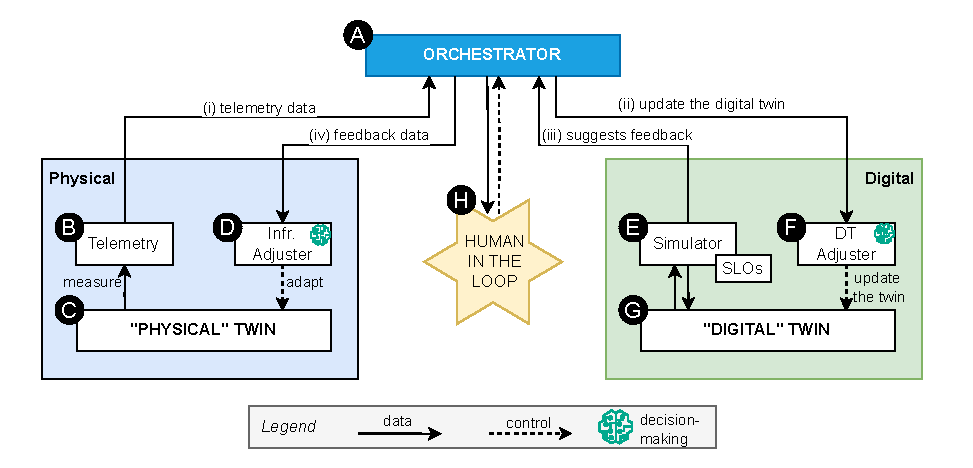
\includegraphics[width=0.95\linewidth]{report/figures/DT-reference-architecture.pdf}
%     \caption{§3 Design. The first reference architecture of a Digital Twin.}
%     \label{fig:placeholder}
% \end{figure}